%%%%%%%%%%%%%%
%
% $Autor: Wings $
% $Project: 
% $Datum: 15.03.2025 $
% $filename: SensorHumidity $
% $Short description: Detaillierte Hardwarebeschreibung des Feuchtigkeitssensors 
% !TeX spellcheck = en_GB/de_DE
% !TeX encoding = utf8
% !TeX root = filename 
% !TeX TXS-program:bibliography = txs:///biber
%
%%%%%%%%%%%%

\chapter{Kapazitiver Feuchtigkeitssensor}

	\section{Feuchtigkeitssensoren Allgemein}
		Sensoren sind technische Bauteile, die chemische, physikalische oder nicht – elektrische Größen erfassen und in ein elektrisches Signal umwandeln. Sie bestehen hauptsächlich aus zwei Komponenten. Eine Komponente ist das Sensor – Element, in welches die gemessenen Eingangsgrößen in elektrische Ausgangssignale umgewandelt werden. Die zweite Komponente ist die Auswerte – Elektronik. Diese sorgt dafür, dass die Ausgangssignale durch die Schaltungselektronik oder durch Softwareprogramme bearbeitet werden und für die Auswertung und Steuerung zur Verfügung stehen. In modernen Sensoren sind diese beiden Komponenten häufig in einem kompakten System vereint. Diese modernen Sensoren werden als intelligente oder smarte Sensoren bezeichnet.
		 
		\vspace{1\baselineskip}
				
		Man unterscheidet zwischen aktiven und passiven Sensoren. Die aktiven Sensoren erzeugen direkt aus der Messgröße ein elektrisches Signal, ohne dass eine zusätzliche Energiezufuhr notwendig ist. Während passive Sensoren eine externe Hilfsspannung benötigen, um ein Signal umzuwandeln
		\cite{Hering:2023}
		
		\vspace{1\baselineskip}
		
		Feuchtigkeitssensoren sind ein spezieller Fall solcher Sensoren, die die Menge an Wasser in einem bestimmten Medium, wie beispielsweise Luft oder Boden, messen und in ein elektrisches Signal umwandeln. Diese Sensoren funktionieren nach verschiedenen physikalischen Verfahren. Sie können durch die Messung von Änderungen der Kapazität, des elektrischen Widerstands oder der Leitfähigkeit eines Materials den Feuchtigkeitsgehalt erfassen.
		\cite{Farahani:2014}

		\vspace{1\baselineskip}

		\textbf{Feuchtigkeitssensoren lassen sich in 2 Typen unterteilen:  } 
		\begin{itemize}
			\item Kapazitive Feuchtigkeitssensoren
			
			\item Resistive Feuchtigkeitssensoren	
		\end{itemize}
		
		Kapazitive Sensoren sind mit zwei isolierten Messelektroden ausgestattet. Je nach Bauweise verfügen sie auch über eine Schutzschicht, die die Elektroden vor Schmutz und Korrosion schützt. Diese Schutzschicht verhindert die Bildung von Oxidationsschichten und macht den Sensor robust und langlebig. 
		
		\vspace{1\baselineskip}
		
		Die kapazitiven Sensoren messen die Änderung der Kapazität zwischen den beiden Elektroden. Diese Veränderung wird durch die Feuchtigkeit verursacht. Das kapazitive Messprinzip beruht darauf, wie stark das Material um die Elektroden herum die elektrischen Felder bzw. dessen Dielektrizitätskonstanten beeinflussen. Im Gegensatz zu trockener Erde, kann Wasser elektrische Felder viel stärker beeinflussen. Dadurch erhöht sich bei mehr Feuchtigkeit die elektrische Kapazität zwischen den Elektroden. Dies wird vom Sensor erkannt und in ein elektrisches Signal umgewandelt. 
		
		\vspace{1\baselineskip}
		
		Resistive Sensoren hingegen messen die Änderung des elektrischen Widerstands. Bei Kontakt mit Feuchtigkeit wird der Widerstand geringer, da Wasser die Leitfähigkeit des Materials erhöht. Diese Sensoren arbeiten mit offenliegenden Elektroden, die direkten Kontakt zum Medium haben, was sie korrosionsanfällig macht. Aufgrund dessen sind resistive Sensoren weniger robust und können schneller beschädigt werden. \cite{Hesse:2014} \cite{Farahani:2014}
		
		\vspace{1\baselineskip}
		
		\textbf{Anwendungen}
		Der Feuchtigkeitssensor findet sowohl in technischen als auch in alltäglichen Situationen Anwendung:
		\cite{Marcinkowska:2023}
		
		\begin{itemize}
			\item \textbf{Landwirtschaft:} In der Landwirtschaft werden Feuchtigkeitssensoren eingesetzt, um die Bodenfeuchte zu überwachen und 
			dadurch eine genaue Bewässerung zu ermöglichen.
			
			\item \textbf{Wetterforschung:}	In der Wetterforschung werden sie eingesetzt, um die Luftfeuchtigkeit zu messen und so eine Wetterprognose aufstellen zu können.  
			
			\item \textbf{Industrie:}In der Industrie helfen sie die Qualität von Materialien wie beispielsweise Holz sicherzustellen, indem sie dessen Feuchtigkeit messen.  
			
			\item \textbf{Haushalt:}Auch im Haushalt finden Feuchtigkeitssensoren Anwendung, wie beispielsweise in Klimaanlagen. 
		\end{itemize}
		
		\vspace{1\baselineskip}
		
		
	\section{Grove-Feuchtigkeitssensor}
		Die Feuchtigkeit beschreibt allgemein den Anteil von Wasser, der in einem gasförmigen, flüssigen oder festen Stoff vorhanden ist. Man spricht von „feucht“, wenn der Wassergehalt eines Stoffes einen festgelegten Schwellenwert überschreitet. In der Thermodynamik liegt der Bereich für die Luftfeuchtigkeit zwischen 0 und ca. 0,03 kg Wasserdampf pro 1 kg trockener Luft.
		\cite{Stephan:2017}
		
		\vspace{1\baselineskip}
		
		Bezogen auf die Bodenfeuchtigkeit beschreibt der Begriff die Menge an Wasser, die in der Erde gespeichert ist und für die Pflanze zur Verfügung steht. Hierbei gibt es jedoch keinen allgemein festgelegten Wert, bei dem die Erde als „feucht“ gilt, da dies von einigen Faktoren wie vom Bodentyp, den klimatischen Bedingungen oder der Pflanzenart abhängt.
		\cite{METER:2023} \cite{Hulatt:2014}
		
		\vspace{1\baselineskip}
		
		Im Rahmen unseres Projekts verwenden wir den Grove – kapazitiven, korrosionsbeständigen Feuchtigkeitssensor von Seeed Studio, um die Feuchtigkeit der Erde im Pflanzentopf zu messen. Dieser Sensor nutzt das kapazitive Messprinzip, um den Feuchtegehalt des Bodens zu erfassen. Er verfügt über zwei isolierte Messelektroden, die auf der Leiterplatte nebeneinander angeordnet sind.  Eine Schutzschicht sorgt dafür, dass die Elektroden keinen direkten Kontakt mit der Erde haben und somit vor Oxidation geschützt sind. Dies macht den Sensor robust und korrosionsbeständig, sodass er sich besonders gut für längere Einsätze in feuchten Umgebungen eignet. Zudem entfallen durch seine Robustheit und Korrosionsbeständigkeit regelmäßige Wartungsarbeiten. \cite{Hesse:2014} \cite{Farahani:2014}
		
		\begin{figure}[h]
			\centering
				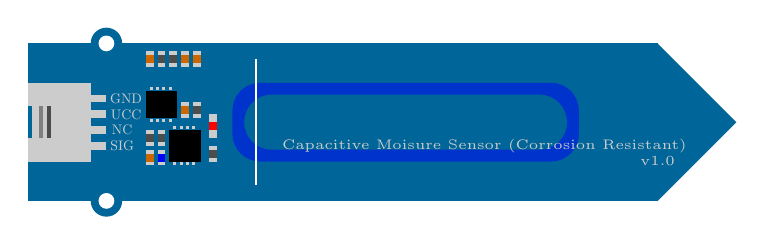
\begin{tikzpicture} 
					% Rechteckiger Hauptteil (8 cm lang, 2 cm breit)
					\fill[blue!60!green] (0,0) rectangle (8,2);
		
					% Koordinaten des Dreiecks
					\fill[blue!60!green] (8,0) -- (8,2) -- (9,1) -- cycle; 
		
					%Bohrungen
					\fill[blue!60!green] (1,2) circle (0.2);
					\fill[blue!60!green] (1,0) circle (0.2);
					\fill [white] (1,2) circle (0.1);
					\fill [white] (1,0) circle (0.1);
		
					%Anschluss
					\fill[white!80!black] (0,0.5) rectangle (0.8,1.5);
					\fill [white!30!black] (0.25,0.8) rectangle (0.3,1.2);
					\fill [white!50!black] (0.15,0.8) rectangle (0.2,1.2);
					\fill [blue!60!green] (0,0.8) rectangle (0.05,1.2);
		
					%Pins
					\fill[white!80!black] (0.8,1.25) rectangle (1,1.35);
					\fill[white!80!black] (0.8,1.05) rectangle (1,1.15);
					\fill[white!80!black] (0.8,0.85) rectangle (1,0.95);
					\fill[white!80!black] (0.8,0.65) rectangle (1,0.75);
		
					\fill [white!80!black] (1.5,1.7) rectangle(1.6,1.9);
					\fill [white!80!black] (1.65,1.7) rectangle(1.75,1.9);
					\fill [white!80!black] (1.8,1.7) rectangle(1.9,1.9);
					\fill [white!80!black] (1.95,1.7) rectangle(2.05,1.9);
					\fill [white!80!black] (2.1,1.7) rectangle(2.2,1.9);
		
					\fill [orange!80!black] (1.5,1.75) rectangle(1.6,1.85);
					\fill [white!30!black] (1.65,1.75) rectangle(1.75,1.85);
					\fill [white!30!black] (1.8,1.75) rectangle(1.9,1.85);
					\fill [orange!80!black] (1.95,1.75) rectangle(2.05,1.85);
					\fill [orange!80!black] (2.1,1.75) rectangle(2.2,1.85);
		
		
					\fill [white!80!black] (1.5,0.7) rectangle(1.6,0.9);
					\fill [white!30!black] (1.5,0.75) rectangle(1.6,0.85);
		
					\fill [white!80!black] (1.65,0.7) rectangle(1.75,0.9);
					\fill [white!30!black] (1.65,0.75) rectangle(1.75,0.85);
		
		
					\fill [white!80!black] (1.5,0.45) rectangle(1.6,0.65);
					\fill [orange!80!black] (1.5,0.5) rectangle(1.6,0.6);
		
					\fill [white!80!black] (1.65,0.45) rectangle(1.75,0.65);
					\fill [blue] (1.65,0.5) rectangle(1.75,0.6);
		
					\fill[white!80!black] (1.95,1.05) rectangle (2.05,1.25);
					\fill[orange!80!black] (1.95,1.1) rectangle (2.05,1.2);
		
					\fill[white!80!black] (2.1,1.05) rectangle (2.2,1.25);
					\fill[white!30!black] (2.1,1.1) rectangle (2.2,1.2);
		
		
					\fill[white!80!black] (2.3,1.1) rectangle (2.4,0.8);
					\fill[red] (2.3,1) rectangle (2.4,0.9);
		
					\fill[white!80!black] (2.3,0.5) rectangle (2.4,0.7);
					\fill[white!30!black] (2.3,0.55) rectangle (2.4,0.65);
		
					%Operatoren
					\fill[black] (1.5,1.05) rectangle (1.9,1.4);
		
					\fill[white!80!black] (1.55,1.41) rectangle (1.59,1.45);
					\fill[white!80!black] (1.63,1.41) rectangle (1.67,1.45);
					\fill[white!80!black] (1.71,1.41) rectangle (1.75,1.45);
					\fill[white!80!black] (1.79,1.41) rectangle (1.83,1.45);
		
					\fill[white!80!black] (1.55,1) rectangle (1.59,1.04);
					\fill[white!80!black] (1.63,1) rectangle (1.67,1.04);
					\fill[white!80!black] (1.71,1) rectangle (1.75,1.04);
					\fill[white!80!black] (1.79,1) rectangle (1.83,1.04);
		
					\fill[black] (1.8,0.5) rectangle (2.2,0.9);
		
					\fill[white!80!black] (1.85,0.91) rectangle (1.89,0.95);
					\fill[white!80!black] (1.93,0.91) rectangle (1.97,0.95);
					\fill[white!80!black] (2.01,0.91) rectangle (2.05,0.95);
					\fill[white!80!black] (2.09,0.91) rectangle (2.13,0.95);
		
					\fill[white!80!black] (1.85,0.49) rectangle (1.89,0.45);
					\fill[white!80!black] (1.93,0.49) rectangle (1.97,0.45);
					\fill[white!80!black] (2.01,0.49) rectangle (2.05,0.45);
					\fill[white!80!black] (2.09,0.49) rectangle (2.13,0.45);
		
					%Oberfläche
					\fill [blue!80!green,rounded corners=10pt] (2.6,0.5) rectangle (7,1.5);
		
					\fill [blue!60!green,rounded corners=10pt] (2.75,0.65) rectangle (6.85,1.35);
					\draw[white] (2.9,0.2) -- (2.9,1.8);
		
					%text der Pins am Anschluss 
					\node [white!80!black] at (1.25,1.3) {\scalebox{0.5}{GND}};
					\node [white!80!black] at (1.25,1.1) {\scalebox{0.5}{UCC}};
					\node [white!80!black] at (1.2,0.9) {\scalebox{0.5}{NC}};
					\node [white!80!black] at (1.2,0.7) {\scalebox{0.5}{SIG}};
		
					%Text auf der Oberfläche 
					\node [white!80!black, font=\tiny] at (5.8,0.7) {Capacitive Moisure Sensor (Corrosion Resistant)};
					\node [white!80!black, font=\tiny] at (8,0.5) {v1.0};
		
				\end{tikzpicture}
			\caption{Grove - Feuchtigkeitssensor nach \cite{Seeed_Datasheet:2019}}
			\label{fig:GroveFeuchtigkeitssensor}
		\end{figure}


	\section{Spezifikationen}
		Die Betriebsspannung des Grove Feuchtigkeitssensors von Seeed Studio liegt zwischen 3,3V und 5V. Dies ermöglicht eine direkte Verbindung mit dem Arduino Nano 33 BLE Sense Lite. Der Anschluss erfolgt über eine Grove – kompatible analoge Schnittstelle, die eine einfache Integration mit Mikrocontrollern ermöglicht. Die Größe des Sensors beträgt 92 x 23,5 x 6,5mm \cite{Seeed_Datasheet:2019}.

		\vspace{1\baselineskip}

		Wie in Abbildung \ref{fig:GroveFeuchtigkeitssensor} zu sehen, verfügt der Grove Feuchtigkeitssensor von Seeed Studio über vier Hauptanschlüsse:
		\cite{Huang:2023}
		
		\begin{itemize}
			\item Signal \textbf{SIG}: Der SIG–Pin liefert das analoge Ausgangssignal des Sensors, welches direkt mit der Bodenfeuchtigkeit verknüpft ist. Je höher die Feuchtigkeit der Erde, desto höher die Spannung, die am SIG–Pin ausgegeben wird. Das ausgegebene Signal wird vom Mikrocontroller erfasst und verarbeitet. So kann der Feuchtigkeitsgehalt der Erde ermittelt werden.
			 
			\item \textbf{NC:} Der NC – Pin ist physisch vorhanden, jedoch intern nicht mit der Schaltung verbunden und hat keine aktive Funktion im Sensor.  
			
			\item \textbf{VCC:} Der \ac{vcc} – Pin versorgt den Sensor mit der notwendigen Betriebsspannung. Der Sensor kann mit 3,3V oder 5V betrieben werden. In unserem Fall wird er mit 3,3V betrieben, da unser Mikrocontroller, der Arduino Nano 33 BLE Sense Lite, 3,3V bereitstellt. 
			
			\item \textbf{GND:} Der GND – Pin fungiert als Masseanschluss des Sensors. Das heißt er ist für die Verbindung zwischen dem Mikrocontroller und dem Nullpotenzial (0V) des Systems zuständig und stellt eine gemeinsame elektrische Referenz für alle Bauteile her. Somit wird eine stabile Signalverarbeitung ermöglicht und der Stromkreis kann korrekt abgeschlossen werden.
		\end{itemize}
		
		Der Grove Feuchtigkeitssensor beinhaltet zusätzlich den LMV358ID - Operationsverstärker, der für die Verstärkung des analogen Signals zuständig ist. Das vom Sensor erzeugte Signal ist oft zu schwach, um direkt vom Mikrocontroller erfasst zu werden. Daher wird der Operationsverstärker eingesetzt, um dieses Signal zu verstärken, sodass es eindeutig und zuverlässig vom Mikrocontroller verarbeitet werden kann. \cite{Texas:2023a}

		\vspace{1\baselineskip}

		Ein weiterer Bestandteil des Grove – Feuchtigkeitssensors ist der integrierte Schaltkreis NE555DR, der für die Signalverarbeitung zuständig ist. Er verarbeitet die kapazitiven Messwerte des Sensors und wandelt diese in ein analoges Spannungssignal um. Die Spannungsausgabe erfolgt dabei umgekehrt proportional zur Bodenfeuchtigkeit. Das heißt je trockener die Erde, desto höher ist der Ausgangswert und bei zunehmender Feuchtigkeit sinkt die Spannung. Es handelt sich hierbei um eine qualitative Messung, die sich gut dazu eignet, anhand eines definierten Schwellwerts zu entscheiden, ob eine Bewässerung notwendig ist.
		\cite{Texas:2016b}

		\vspace{1\baselineskip}

		Der Grove Feuchtigkeitssensor wird laut Seeed Studio in verschiedenen Bereichen eingesetzt, darunter im botanischen Gartenbau, in der Feuchtigkeitssensorik und in der Konsistenzmessung.
		\cite{Seeed_Datasheet:2019}
		
		Der Sensor liefert ein analoges Spannungssignal im Bereich von 0V bis 3,3V. Diese Spannung wird vom integrierten Analog-Digital-Wandler (\ac{adc}) des Mikrocontrollers mit einer 10-Bit-Auflösung in einen digitalen Integerwert zwischen 0 und 1023 umgewandelt. \cite{ArduinoReadAnalogeVoltage:2024} \cite{Bartlett:2023}
		
		
	\section{Bibliotheken}
		In der Arduino-Umgebung können die Funktionen durch den Einsatz zahlreicher Bibliotheken (Libraries) erweitert werden. Diese Bibliotheken bieten vorgefertigte Code-Sammlungen, die speziell entwickelt wurden, um die Programmierung bestimmter Komponenten oder Funktionen zu vereinfachen. Statt den gesamten Code für eine bestimmte Aufgabe selbst zu schreiben, kann der Entwickler die passende Bibliothek einbinden und so auf eine Vielzahl von bereits programmierten Funktionen zugreifen. Bibliotheken bieten eine effiziente Möglichkeit, gängige Aufgaben wie die Ansteuerung von Sensoren, Motoren oder Displays durch einfache Funktionsaufrufe zu erledigen, ohne den Code dafür von Grund auf neu schreiben zu müssen.
		\cite{Söderby:2024} \cite{SöderbyundHylen:2024} \cite{Barber:2020}
		
		
		\subsection{Beschreibung}
			Für den in diesem Projekt verwendeten kapazitiven Bodenfeuchtesensor ist keine spezielle Bibliothek erforderlich, da der Sensor über einen analogen Ausgang arbeitet. Der Sensor gibt den Feuchtigkeitswert als analoge Spannung aus, welche der Mikrocontroller mit der \PYTHON{analogRead()} – Funktion einlesen kann.  

			\vspace{1\baselineskip}

			Das Board vom Arduino ist mit einem 12-Bit-Analog-Digital-Wandler (\ac{adc}) ausgestattet, welcher dafür sorgt, dass die Eingangsspannungen zwischen 0 – 3,3 V auf Integer Werte zwischen 0 – 4095 gewandelt werden. Diese sind proportional zu Bodenfeuchte, wobei höhere Werte eine höhere Spannung und somit auch höhere Integer-Werte zurückgeben. Umgekehrt liefert ein trockener Boden einen geringeren Spannungswert, was in einem geringeren Messwert resultiert. \cite{Bartlett:2023}

			\vspace{1\baselineskip}

			Mit der Funktion \PYTHON{analogRead()} wird diese analoge Spannung ausgelesen und es wird ein entsprechender digitaler Wert zurückgegeben. Durch diese Schnittstelle lässt sich der Sensor direkt in das Projekt einbinden, ohne Gebrauch einer zusätzlichen Bibliothek zu machen. Dadurch wird Speicherplatz gespart und die reduzierte Komplexität des Codes macht die Programmierung einsteigerfreundlich und übersichtlich. \cite{Bartlett:2023}

			\vspace{1\baselineskip}

			Die Sensorwerte werden mit Hilfe der seriellen Schnittstelle \PYTHON{Serial.print()} und \PYTHON{Serial.println()} ausgegeben. Die Funktion \PYTHON{Serial.print()} gibt den Text ohne einen Zeilenumbruch in lesbaren ASCII-Zeichen aus, während die Funktion \PYTHON{Serial.println()} einen Zeilenumbruch inkludiert. Die ausgegebenen Werte können über die Arduino \ac{ide} überwacht werden und zur automatischen Steuerung von Aktoren genutzt oder per Bluetooth Low Energy (BLE) an die App übertragen werden.
			\cite{SunFounder:2025} \cite{Arduino:2024}


	\section{Kalibrieren}
		Da der Schwellenwert für die Bodenfeuchtigkeit je nach Bodentyp, Pflanzenart und Umgebungsbedingungen stark variiert und es somit keinen allgemeinen festgelegten Referenzwert gibt, wurde der Sensor manuell kalibriert. Ziel war es, realistische Wertebereiche für trocken und feucht zu bestimmen.
		
		\vspace{1\baselineskip}
		
		Der Sensor liefert ein analoges Spannungssignal, das vom Analog-Digital-Wandler (\ac{adc}) des Mikrocontrollers in digitale Werte zwischen 0 und 1023 umgewandelt wird. Diese werden im Programmcode auf eine prozentuale Skala von 0 Prozent (sehr trocken) bis 100 Prozent (sehr feucht) umgerechnet. Zur Überprüfung und Beobachtung der Messdaten wurde das System über Bluetooth mit der App nRF Connect verbunden, über die die aktuellen Feuchtigkeitswerte in Prozent angezeigt und abgelesen werden konnten. \cite{Arduino:2024}
		
		\vspace{1\baselineskip}
		
		Für die Kalibrierung wurde die Pflanze zunächst über mehrere Tage hinweg bei Zimmertemperatur nicht bewässert, bis die Erde deutlich ausgetrocknet war (Abbildung \ref{fig:TrockeneErde}). Um diesen Zustand zu überprüfen, wurde zusätzlich der sogenannte Fingertest durchgeführt. Dabei wird ein Finger etwa 2 bis 3 Zentimeter tief in die Erde gesteckt. Bleibt beim Herausziehen keine Erde am Finger haften, gilt der Boden als zu trocken und sollte bewässert werden. In diesem Zustand wurden vom Sensor Werte zwischen 36 Prozent und 39 Prozent erfasst (Abbildung \ref{fig:TrockeneWerte}). \cite{Sharma:2024}
		
		\begin{figure}[h]
			\centering
			
\includegraphics[width=7cm]{Sensor/Humidity/SensorTopf.png}
			\caption{Blumentopf mit trockener Erde [Eigene Darstellung]}
			\label{fig:TrockeneErde}
		\end{figure}
		
		\begin{figure}[h]
			\centering
			
\includegraphics[width=5cm]{Sensor/Humidity/AppValues.jpeg}
			\caption{Feuchtigkeitswerte bei trockener Erde [Eigene Darstellung]}
			\label{fig:TrockeneWerte}
		\end{figure}
		
		\clearpage
		
		Anschließend wurde die Pflanze gezielt so weit gegossen, dass die Erde als leicht feucht beurteilt werden konnte. Die dabei gemessenen Werte lagen zwischen 47 Prozent und 51 Prozent (Abbildung \ref{fig:NasseErde}). Als Schwellenwert wurde daraufhin ein Mittelwert festgelegt. Dieser wurde im Programmcode auf einen Integerwert von 550 gesetzt, was ungefähr 42 Prozent  Bodenfeuchtigkeit entspricht. Wird dieser Wert unterschritten, so wird eine automatische Bewässerung ausgelöst (Abbildung \ref{fig:NassWerte}). Liegt der Messwert darüber, bleibt die Wasserzufuhr deaktiviert.
		
		\begin{figure}[h]
			\centering
			
\includegraphics[width=7cm]{Sensor/Humidity/SensorTopfNass.png}
			\caption{Blumentopf mit nasser Erde [Eigene Darstellung]}
			\label{fig:NasseErde}
		\end{figure}
		
		\begin{figure}[h]
			\centering
			
\includegraphics[width=5cm]{Sensor/Humidity/AppValuesNass.jpeg}
			\caption{Feuchtigkeitswerte bei nasser Erde [Eigene Darstellung]}
			\label{fig:NassWerte}
		\end{figure}
		
		\clearpage
	
	
	\section{Codebeispiel}
		Dieser Abschnitt stellt einen Beispielcode für die Nutzung des Grove Feuchtigkeitssensors von Seeed Studio bereit. Der Code liest kontinuierlich die analogen Werte vom Sensor aus und gibt diese über die serielle Schnittstelle aus. Mit Hilfe dieses Codes, kann die Sensorfunktion überprüft und der Feuchtigkeitswert des Bodens in Echtzeit überwacht werden.
		
		\vspace{1\baselineskip}
		
		Im Code werden grundlegende Arduino – Funktionen verwendet, die bereits im vorherigen Abschnitt erläutert wurden, wie beispielsweise die Initialisierung der seriellen Schnittstelle im Setup, das Einlesen des analogen Signals mit \PYTHON{analogRead()} und die Ausgabe der Werte über \PYTHON{Serial.print()} bzw. \PYTHON{Serial.println()}. Eine kurze Pause zwischen den Messungen wird durch den Befehl \PYTHON{delay()} eingefügt.
		
		\begin{center}
			\captionof{figure}{Beispielcode}
			\ArduinoExternal{}{../../Code/Arduino/Humidity/Sample/Sample.ino}
			\label{Code:Beispielcode}
		\end{center}


	\section{Anwendung}
		Basierend auf der zuvor beschriebenen Kalibrierung des Sensors mit einem Schwellwert von 550, wird in diesem Abschnitt eine einfache Anwendung vorgestellt, die den Bodenfeuchtigkeitswert kontinuierlich misst und daraufhin die Pumpe steuert. Der Sensor ist dabei an den analogen Eingang A6 angeschlossen.
		Der Code liest kontinuierlich den analogen Wert des Sensors aus. Liegt der gemessene Wert unterhalb des festgelegten Schwellwerts von 550, wird die Pumpe aktiviert. Sobald der Sensorwert den Schwellwert erreicht oder überschreitet, schaltet die Pumpe wieder aus.
		Diese einfache Steuerung ermöglicht eine automatisierte Bewässerung, die auf den realen Feuchtigkeitswerten des Bodens basiert. Durch das regelmäßige Auslesen und Auswerten des Sensorsignals wird eine präzise Bewässerung sichergestellt, was zudem auch Wasser spart. 
		Der hier vorgestellte Code dient als Grundlage für weiterführende Anwendungen, in denen beispielsweise zusätzliche Sensoren integriert werden können.
		
		\cite{Arduino3}
		\begin{center}
			\captionof{figure}{Einfache Anwendung}
			\ArduinoExternal{}{../../Code/Arduino/Humidity/SimpleApp/SimpleApp.ino}
			\label{Code:Anwendung}
		\end{center}


	\section{Tests}
		Nach der Kalibrierung wurde das System getestet, um die Funktionsfähigkeit zu überprüfen. Dabei wurde beobachtet, ob die Pumpe korrekt reagiert, sobald der definierte Schwellenwert von 550 unterschritten oder überschritten wird. 
		
		
	\section{Weiterführende Literatur}
		Huang, Jianjing (2023): Grove – Capacitive Moisture Sensor (Corrosion Resistant), Verfügbar unter:  \href{https://wiki.seeedstudio.com/Grove-Capacitive_Moisture_Sensor-Corrosion-Resistant}{wiki.seeedstudio.com/Grove-CapacitiveMoistureSensor-Corrosion-Resistant} [abgerufen am 04.04.2025]
		
		\begin{itemize}
			\item Eine übersichtliche Einführung in die Eigenschaften und die Nutzung des kapazitiven Grove – Feuchtigkeitssensors von Seeed Studio. Es wird die Korrosionsbeständigkeit im Vergleich zu resistiven Sensoren beschrieben und es werden praktische Beispiele für den Einsatz mit Mikrocontrollern gennant. 
		\end{itemize}

		\vspace{1\baselineskip}

		 Abdelmoneim, Ahmed A. et. al. (2025): Comparative Analysis of Soil Moisture- and Weather-Based Irrigation Scheduling for Drip-Irrigated Lettuce Using Low-Cost Internet of Things Capacitive Sensors, Verfügbar unter: \href{https://www.researchgate.net/publication/389563237}{Researchgate Publikation: 389563237}  [abgerufen am 29.04.2025] 
		 
		 \vspace{1\baselineskip}
		 		
		 Hrisko, Joshua (2020): Capacitive Soil Moisture Sensor Theory, Calibration, and Testing, Verfügbar unter: \href{https://www.researchgate.net/publication/342751186}{Researchgate Publikation: 342751186} [abgerufen am 29.04.2025]
		 
		\begin{itemize}
			\item Ein Überblick über aktuelle wissenschaftliche Veröffentlichungen zu kapazitiven Feuchtigkeitssensoren. Thematisiert werden Sensordesign, Materialauswahl, Messgenauigkeit und Anwendungen, insbesondere in der Landwirtschaft.
		\end{itemize}
		
		\vspace{1\baselineskip}
		
		Ekbert Hering und Gert Schönfelder, Sensoren in Wissenschaft und Technik – Funktionsweise und Einsatzgebiete, Springer Vieweg, 2023, ISBN: 9783658394905 \cite{Ekbert:2023} 
		\begin{itemize}
			\item 	Eine umfassende und aktuelle Einführung in die Grundlagen und Anwendungen von Sensoren in Technik, Biologie und Medizin. Das Buch behandelt neben physikalischen Grundlagen auch Themen wie Schnittstellen, Sicherheit und Energieversorgung moderner Sensoren.
		\end{itemize}